\section{Data Types}
The following section will describe each data type that Germinate can handle in more detail. We will describe both the web interface that is used to display this data as well as what the export formats for each of the types are.

\subsection{Passport Data}

\subsubsection{Multi-Crop Passport Descriptors}
The Multi-Crop Passport Descriptors (MCPD) \cite{mcpd} is a widely used international standard to facilitate germplasm passport information exchange defined by the FAO. Germinate is fully MCPD V.2.1 compatible. The MCPD standard is used by many genebanks and genetic resources tools and utilities.

\subsection{Genotypic Data}
When we talk about genotypic data in the context of Germinate, we are referring to Single Nucleotide Polymorphic (SNP) or Simple sequence repeat (SSR) data. The data export process is shown in Figure \ref{fig:features:group-subselection}. After selecting the dataset you want to export, you can decide which accessions and markers should be included in the output. Data can be exported against different maps (cf. Section \ref{sec:features:genotypic-maps}), e.g. physical vs. genetic marker positions.

The data is exported into a tab-delimited text format as well as Flapjack \cite{flapjack} format. Figure \ref{fig:features:genotypic-data-flapjack} shows an example of data exported from Germinate visualized in Flapjack.

\begin{figure}
	\centering
	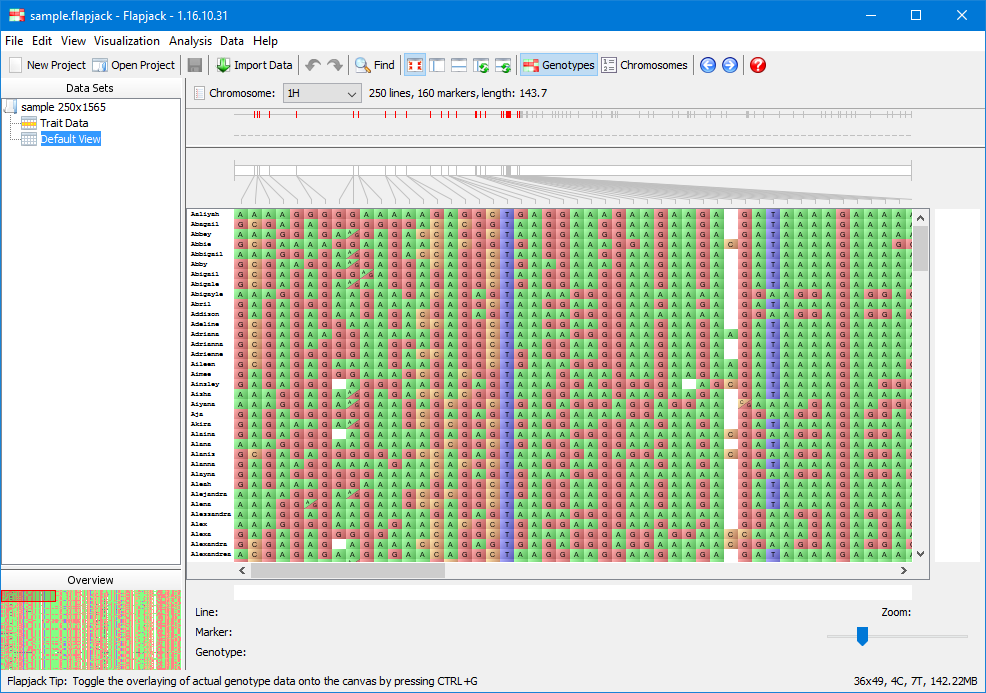
\includegraphics[width=0.85\linewidth]{img/features/genotypic-data-flapjack.png}
	\caption{Genotypic data exported from Germinate and visualized in Flapjack.}
	\label{fig:features:genotypic-data-flapjack}
\end{figure}

\subsubsection{Allele Frequency Data}
\todo{Paul}

\subsubsection{Genotypic Maps}
\label{sec:features:genotypic-maps}

\subsubsection{Genetic Markers}

\subsection{Phenotypic Trials Data}
Phenotypic data is a big part of Germinate. We put a lot of effort into developing meaningful visualizations as well as functionality and interoperability with our other software tools. 

After selecting a dataset (or multiple datasets), you will have the choice between different visualizations and the data download. The first tab shows an overview over the data within the selected datasets, whereas the second tab lets you plot two phenotypes against each other in a scatter plot. This is particularly useful to see if there is any correlation between them. Hovering over data points shows the values per dimension as well as the accession that is responsible for this data point. Clicking on this data point will take you to the passport page for this accession. You can draw a shape around data points of interest by clicking and dragging the mouse across the chart. This will highlight the data points within the shape. You can then either right-click or use the icon in the top right of the chart to add/remove these items to/from the marked item list.

\subsection{Climate Data}

\subsection{Chemical Compound Data}